% !TeX root = widefieldscan.tex
\svnidlong
{$HeadURL$}
{$LastChangedDate$}
{$LastChangedRevision$}
{$LastChangedBy$}

\section{Results}\label{sec:Results}
\subsection{Image Merging and Reconstruction}\label{sec:Image Merging and Reconstruction}
Figure~\ref{fig:wide-field-scan-results}(a) shows corrected projections from three overlapping subscans prior to merging, including regions where the subscans are overlapping. Figure~\ref{fig:wide-field-scan-results}(b) shows one merged projection prior to reconstruction and Figure~\ref{fig:wide-field-scan-results}(c) shows one slice of the reconstructed dataset. In Figure~\ref{fig:wide-field-scan-results} protocol B is show, because it was scanned using the highest number of projections. A reconstructed slice covers a field of view of 2792$\times$2792 pixels (4.13$\times$\SI{4.13}{\milli\meter}), which is almost three times the size of what can be achieved with one single binned scan (1024 pixels or \SI{1.52}{\milli\meter}). %1024 * 1.48 um/px = 1.51552mm
The dashed circles on the reconstructed slice mark the start and the end of the overlap region.

\begin{figure}
	\centering
	\caption{Workflow of a wide field scan. The images show a rat lung sample from a Sprague-Dawley rat, obtained 21 days after birth, scanned with the acquisition protocol B (Table~\ref{tab:protocols}). %
			(a) Three corrected and independently acquired projections from subscans $s_1$--$s_3$ are shown. Each one is 1024\(\times\)1024 pixels large and covers a field of view of \SI{1.52}{\milli\meter}. Subscans $s_1$ and $s_2$ overlap by 141 pixels (red and green overlay), subscans $s_2$ and $s_3$ overlap by 138 pixels (blue and yellow overlay). %
			(b) Merged projection obtained from the three subscans shown in subfigure (a). Each merged projection has a size of 2792\(\times\)1024 pixels. Due to the overlap required to merge the projections, the width of the merged projections is slightly smaller than three times the width of the subscans. %
			(c) Cropped slice of the reconstructed tomographic dataset. The dashed red circles mark the start and end of the overlap region.}
	\ifiucr
		%\documentclass{article}
%\usepackage{subfig}
%\usepackage{tikz}
%\usepackage{siunitx}
%\begin{document}
%\newcommand{\imsize}{\linewidth}
%\newlength\imagewidth % needed for scalebars
%\newlength\imagescale % needed for scalebars
%\begin{figure}
%	\centering
%%%%%%%%%%%%%%%%%%%%%%%%%%%%%
	\renewcommand{\imsize}{.333\linewidth}
	\pgfmathsetlength{\imagewidth}{\imsize} % desired display width of image
	\pgfmathsetlength{\imagescale}{\imagewidth/1024} % pixel width of image
			% --------------------------------------------------------------
			% Cutline between SubScan 1 and 2: 141 pixels
			% Cutline between SubScan 2 and 3: 138 pixels
			% --------------------------------------------------------------
			\def\size{1023}%
			\begin{tikzpicture}[x=\imagescale,y=-\imagescale]%
				\node[anchor=north west,inner sep=0pt,outer sep=0pt] at (0,0)%
					{\includegraphics[width=\imagewidth]{img/merge/R108C21Cb_s13358_normalize}};%
%					{\includegraphics[width=\imagewidth]{R108C21Cb_s13358_normalize}};%
				\def\overlap{141}%
				\fill [red, nearly transparent] (1024-\overlap,1) rectangle (\size,\size);%
				\draw (1024-\overlap,1) rectangle (\size,\size);%
				\node [anchor=center, color=white] at (100,1024-100) {a)};				
			\end{tikzpicture}%
			\begin{tikzpicture}[x=\imagescale,y=-\imagescale]%
				\node[anchor=north west,inner sep=0pt,outer sep=0pt] at (0,0)%
					{\includegraphics[width=\imagewidth]{img/merge/R108C21Cb_s23358_normalize}};%
%					{\includegraphics[width=\imagewidth]{R108C21Cb_s23358_normalize}};%
				\def\overlap{141}%
				\fill [green, nearly transparent] (1,1) rectangle (\overlap,\size);%
				\draw (1,1) rectangle (\overlap,\size);%
				\def\overlap{138}%
				\fill [blue, nearly transparent] (1024-\overlap,1) rectangle (\size,\size);%
				\draw (1024-\overlap,1) rectangle (\size,\size);%
			\end{tikzpicture}%
			\begin{tikzpicture}[x=\imagescale,y=-\imagescale]%
				% place image (integer coordinates refer to pixel centers):
				\node[anchor=north west,inner sep=0pt,outer sep=0pt] at (0,0)%
					{\includegraphics[width=\imagewidth]{img/merge/R108C21Cb_s33358_normalize}};%
%					{\includegraphics[width=\imagewidth]{R108C21Cb_s33358_normalize}};%
				\def\overlap{138}%
				\fill [yellow, nearly transparent] (1,1) rectangle (\overlap,\size);%
				\draw (1,1) rectangle (\overlap,\size);%
				\draw[|-|,thick] (5,200) -- (1021,200) node [color=white,midway,above] {\SI{1.51552}{\milli\meter}};%
				\def\x{924}% 1024 - 100
				\def\y{922}% 1024 * .9 = 921.6
				\def\bar{338}% 100 px = 148 um
				\draw[|-|,thick,color=white] (\x-\bar,\y) -- (\x,\y) node [midway,above] {\SI{500}{\micro\meter}};%
			\end{tikzpicture}%
			\label{fig:subscans}%
%%%%%%%%%%%%%%%%%%%%%%%%%%%%%	
%	\caption{caption}
%\end{figure}
%\end{document}\\%
		%\documentclass{article}
%\usepackage{subfig}
%\usepackage{tikz}
%\usepackage{siunitx}
%\begin{document}
%\newcommand{\imsize}{\linewidth}
%\newlength\imagewidth % needed for scalebars
%\newlength\imagescale % needed for scalebars
%\begin{figure}
%	\centering
%%%%%%%%%%%%%%%%%%%%%%%%%%%%%
		\renewcommand{\imsize}{\linewidth}%
		\pgfmathsetlength{\imagewidth}{\imsize} % desired displayed width of image
		\pgfmathsetlength{\imagescale}{\imagewidth/2793}% pixel width of image
			\begin{tikzpicture}[x=\imagescale,y=-\imagescale]%
				\node[anchor=north west,inner sep=0pt,outer sep=0pt] at (0,0)%
					{\includegraphics[width=\imagewidth]{img/merge/R108C21Cb_mrg3333_normalize}};%
%					{\includegraphics[width=\imagewidth]{R108C21Cb_mrg3333_normalize}};%
				\def\x{2693} % 2793-100
				\def\y{922} % 1024*.9 = 921.6
				\def\bar{338} % 100 px = 148 um
				\draw[|-|,thick,color=white] (5,256) -- (2787,256) node [midway,above] {\SI{4.13364}{\milli\meter}};
				\draw[|-|,thick,color=white] (\x-\bar,\y) -- (\x,\y) node [midway,above] {\SI{500}{\micro\meter}};
				\node [anchor=center, color=white] at (100,1024-100) {b)};
				\end{tikzpicture}%
			\label{fig:merge-proj}%
%%%%%%%%%%%%%%%%%%%%%%%%%%%%%	
%	\caption{caption}
%\end{figure}
%\end{document}\\%
		%\documentclass{article}
%\usepackage{subfig}
%\usepackage{tikz}
%\usepackage{siunitx}
%\begin{document}
%\newcommand{\imsize}{\linewidth}
%\newlength\imagewidth % needed for scalebars
%\newlength\imagescale % needed for scalebars
%\begin{figure}
%	\centering
%%%%%%%%%%%%%%%%%%%%%%%%%%%%%
		\pgfmathsetlength{\imagewidth}{\imsize}%
		\pgfmathsetlength{\imagescale}{\imagewidth/2792}%
			\begin{tikzpicture}[x=\imagescale,y=-\imagescale]%
				\node [anchor=north west,inner sep=0pt,outer sep=0pt] at (0,0)%
					{\includegraphics[width=\imagewidth]{img/merge/R108C21Cb_mrg1024rec8bit}};% ``mogrify -shave 0x900 -format png R108C21Cb_mrg1024rec8bit.tif''
%					{\includegraphics[width=\imagewidth]{R108C21Cb_mrg1024rec8bit}};
				\clip (0,0) rectangle (2792,992);				
				\def\x{2692} % 2792-100
				\def\y{893} % 992 * .9 = 892.8
				\def\bar{338} % 100 px = 148 um
				%%%% scalebar
					\draw[|-|,thick,color=white] (\x-\bar,\y) -- (\x,\y) node [midway, above] {\SI{500}{\micro\meter}};
%					\draw[|-|,thick,color=white] (5,30) -- (2787,30) node [midway, below] {\SI{4.13216}{\milli\meter}};
				%%%% big circle
					\draw [dashed, ultra thick, color=red] (2792/2,992/2) circle (512);
					\def\angle{35}
					\draw [white, thick, <->] (2792/2,992/2) +(\angle:0) --  node (bigto) {} +(\angle:512); 
					\node [white] (bigfrom) at (349,256){$\frac{1024}{2}$px};
					\draw [white, ->, thick, densely dotted] (bigfrom) to [bend left=45] (bigto);
				%%%% big circle
				%%%% 141px circle
				\draw [dashed, ultra thick, color=red] (2792/2,992/2) circle (512-141);
				\def\angle{35+90}
					\draw [white,thick,<->] (2792/2,992/2) +(\angle:0) -- node (smallto) {} +(\angle:512-141);
					\node [white] (smallfrom) at (349,384) {$\frac{1024}{2}-141$px};
					\draw [white, ->, thick, densely dotted] (smallfrom) to [bend left=45] (smallto);
				%%%% 141px circle					
%				%%%% 138px circle
%				\draw [dashed,color=red] (2792/2,992/2) circle (512-138);
%				\def\angle{45+90+90}
%					\draw [white,<->] (2792/2,992/2) +(\angle:0) -- node (vsmallto) {} +(\angle:512-138);
%					\node [white] (vsmallfrom) at (2972-768,992-512) {$\frac{1024}{2}-138$px};
%					\draw [white,->,densely dotted] (vsmallfrom) to [bend right=45] (vsmallto);
%				%%%% 138px circle
				%%%% center
				\fill [color=red] (2792/2,992/2) circle (5);
				%%%% center
				%%%% inset
%				\newcommand{\size}{.2\imagewidth}%
%				\clip (256,256) rectangle (512,512);
%				\node[anchor=north west,inner sep=0pt,outer sep=0pt] at (0,0)
%					{\includegraphics[width=\size]{R108C21Cb_mrg1024rec8bit}};
%					\draw[white] (0,0) rectangle (\size,-\size);
				%%%% inset
				\node [anchor=south west, color=white] at (0,990) {(c)};			
				\end{tikzpicture}%
			\label{fig:merge-rec}%
%%%%%%%%%%%%%%%%%%%%%%%%%%%%%	
%	\caption{caption}
%\end{figure}
%\end{document}\\%
	\else
	\fi
	\label{fig:wide-field-scan-results}
\end{figure}

Figure~\ref{fig:s2-wfs} shows the advantages of the wide field acquisition scheme. With---in this particular case---an enlargement of the field of view by almost a factor of three, it is possible to visualize entire acini at high resolution. For a conventional scan (fig.~\ref{fig:s2-wfs}(a)), the airway segments in the sample are only partially contained inside the dataset (magenta and yellow). Semitransparent airway segments are contained in the sample, but are not visible in the field of view of a dataset obtained with a conventional scan. Increasing the field of view (fig.~\ref{fig:s2-wfs}(b)) allows the visualization of those segments to their full extent. A third acinus (cyan) which was not visible in Figure~\ref{fig:s2-wfs}(a) can now easily be visualized.

%\onecolumn
\renewcommand{\imsize}{.618\linewidth}%
\begin{figure}
	\centering
	\caption{Three-dimensional visualization of the distal-medial tip of the right lower rat lung lobe. The gray structure in the background shows a semitransparent view of the tomographic dataset with segmented airways. The foreground shows isosurfaces of terminal airways. The wireframe cube has a side length of 1024 pixels and encloses the field of view of one conventional scan. (a): Conventional scan; the extracted airway segments (magenta and yellow) are only partially contained inside the total sample volume. Airway segments not contained in the dataset, but present in the sample are shown semitransparent. This conventional scan corresponds to a reconstruction of the central of the three wide field scan subscans. (b): Wide field scan with increased field of view; the magenta and yellow segment show entire acini inside the dataset, the cyan segment contains a partially cut acinus. All airway segments inside the sample are contained in the tomographic dataset.}
	\ifiucr
	%%%%%%%%%%%%%%%%%%%
		\pgfmathsetlength{\imagewidth}{\imsize}%
		\pgfmathsetlength{\imagescale}{\imagewidth/1379}%
		\begin{tikzpicture}[x=\imagescale,y=-\imagescale]
			\def\x{852} % scalebar-x at golden ratio of x=1379px
			\def\y{898} % scalebar-y at 90% of height of y=998px
			\node[anchor=north west, inner sep=0pt, outer sep=0pt] at (0,0)
				{\includegraphics[width=\imagewidth]{img/conv_vs_wfs/scan-conventional}};
			% 618px = 1.5155mm > 100px = 245um > 204px = 500um, 41px = 100um
			%\draw[color=red,|-|,thick] (174,761) -- (753,977) node [sloped,midway,above] {\SI{1.5155}{\milli\meter} (1024px)};
			\draw[|-|,thick] (\x,\y) -- (\x+204,\y) node [fill=white, semitransparent, midway, above] {\SI{500}{\micro\meter}};
			\draw[|-|,thick] (\x,\y) -- (\x+204,\y) node [midway, above]{\SI{500}{\micro\meter}};
		\draw[anchor=south west] (0,998) node [fill=white, semitransparent] {(a)} node {(a)};
		\end{tikzpicture}%
	%%%%%%%%%%%%%%%%%%%
		\\%
		\pgfmathsetlength{\imagewidth}{\imsize}%
		\pgfmathsetlength{\imagescale}{\imagewidth/1379}%
		\begin{tikzpicture}[x=\imagescale,y=-\imagescale]
			\def\x{852} % scalebar-x at golden ratio of x=1379px
			\def\y{898} % scalebar-y at 90% of height of y=998px
			\node[anchor=north west, inner sep=0pt, outer sep=0pt] at (0,0)
				{\includegraphics[width=\imagewidth]{img/conv_vs_wfs/scan-widefield}};
			% 620px = 1.5155mm > 100px = 245um > 204px = 500um, 41px = 100um
			%\draw[color=red,|-|,thick] (174,761) -- (755,977) node [sloped,midway,above] {\SI{1.5155}{\milli\meter} (1024px)};
			\draw[|-|,thick] (\x,\y) -- (\x+204,\y) node [fill=white, semitransparent, midway, above] {\SI{500}{\micro\meter}};
			\draw[|-|,thick] (\x,\y) -- (\x+204,\y) node [midway, above]{\SI{500}{\micro\meter}};
			\draw[anchor=south west] (0,998) node [fill=white, semitransparent] {(b)} node {(b)};
		\end{tikzpicture}%
	%%%%%%%%%%%%%%%%%%%
	\else
	\fi
	\label{fig:s2-wfs}
\end{figure}
%\twocolumn

As expected, the calculated quality of the reconstructions representing the different protocols decreases as a function of total number of obtained projections (Figure~\ref{fig:NormalizedErrorPlot}). The calculated error of the different protocols (blue diamonds) shows the experimental results
\cbstart
obtained from actual scans of lung tissue. The plots for the simulation (19 protocols, as defined in section~\ref{sec:quality guided protocols}, red dots) and
\cbend
the normalized difference value are not perfectly in agreement, but show the same trend. The simulation shows an exponential decrease in quality, while the calculated, normalized error shows a more linear decrease in quality from protocol B towards protocol T.

\begin{figure}
	\centering
	\caption{Plot of normalized difference Value ($E_{i_{norm}}$, blue diamonds) for the 19 scanned protocols overlaid over Quality-plot (red dots) obtained from the simulation (described in section~\ref{sec:quality guided protocols}. The normalized Error has been calculated using the difference image of each protocol $i$ with protocol B. The error bars for each protocol show the standard deviation of the error calculated for 205 of the 1024 slices. Note that the scale of the error was normalized to 20--\SI{100}{\percent}, so that both the quality from the simulation and the error are directly comparable. The abscissa shows the scanning time in percentage of time used for the gold standard scan. Protocol T on the far left corresponds to the fastest scanning time, protocol B on the far right to the slowest. The protocols in between are shown from T--B for increasing percentage of the scanning time.}
	\ifiucr		
		%\documentclass{article}
%\usepackage{tikz,pgfplots}
%\usepackage[pdftex,active,tightpage]{preview}
%\begin{document}
%\begin{preview}

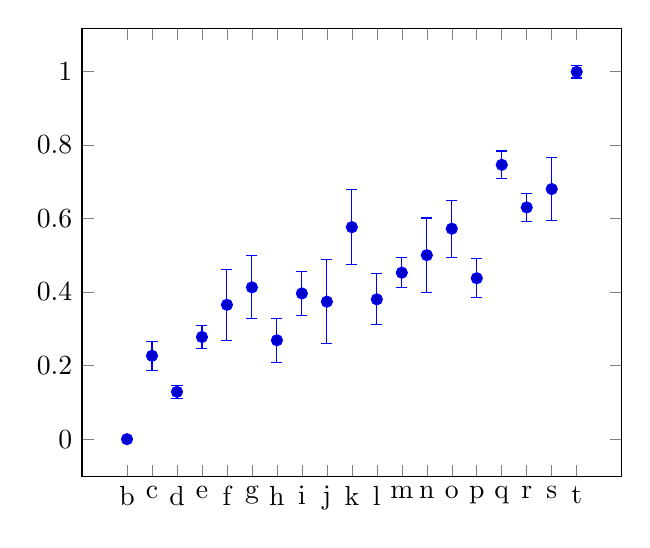
\begin{tikzpicture}
\begin{axis}[%
	%grid=both,%
	%xmajorgrids,%
	xtick={1,2,3,4,5,6,7,8,9,10,11,12,13,14,15,16,17,18,19},%
	xticklabels={b,c,d,e,f,g,h,i,j,k,l,m,n,o,p,q,r,s,t},%
]
% Line plot
\addplot
	plot[ 	%smooth,
	   		only marks,
	      	error bars/.cd,
	      	y dir=both, y explicit %
		]
	coordinates{
	(1,0) 			+- (0,0)
	(2,0.226697)	+- (0,0.0389)
	(3,0.128649)	+- (0,0.0174)
	(4,0.277819)	+- (0,0.0316)
	(5,0.365309) 	+- (0,0.0960)
	(6,0.412726)	+- (0,0.0856)
	(7,0.268849) 	+- (0,0.0598)
	(8,0.396237)	+- (0,0.0589)
	(9,0.373823)	+- (0,0.1148)
	(10,0.576375)	+- (0,0.1020)
	(11,0.380172) 	+- (0,0.0696)
	(12,0.452672)	+- (0,0.0404)
	(13,0.500303)	+- (0,0.1010)
	(14,0.572158)	+- (0,0.0778)
	(15,0.437586)	+- (0,0.0524)
	(16,0.745885)	+- (0,0.0376)
	(17,0.630023)	+- (0,0.0386)
	(18,0.679989)	+- (0,0.0852)
	(19,0.998734)	+- (0,0.0169)
};

\end{axis}
\end{tikzpicture}


% plot erstellt mit MATLAB-File p:\doc\MATLAB\WFS-CompareDMPs\wfs_Compare2008c.m (FromToTo = 1:5:1024)
% und matlab2tikz

%[ 1:19;std(NormCumulativeError);mean(NormCumulativeError)]
%
%ans =
%
%  Columns 1 through 12
%
%    1.0000    2.0000    3.0000    4.0000    5.0000    6.0000    7.0000    8.0000    9.0000   10.0000   11.0000   12.0000
%         0    0.0389    0.0174    0.0316    0.0960    0.0856    0.0598    0.0589    0.1148    0.1020    0.0696    0.0404
%         0    0.2267    0.1286    0.2778    0.3653    0.4127    0.2688    0.3962    0.3738    0.5764    0.3802    0.4527
%
%  Columns 13 through 19
%
%   13.0000   14.0000   15.0000   16.0000   17.0000   18.0000   19.0000
%    0.1010    0.0778    0.0524    0.0376    0.0386    0.0852    0.0169
%    0.5003    0.5722    0.4376    0.7459    0.6300    0.6800    0.9987          	
         	
%
%\end{preview}
%\end{document}
	\else
	\fi
	\label{fig:NormalizedErrorPlot}
\end{figure}

\subsubsection{Three-dimensional visualization of different protocols}
\label{subsec:comparison}
The tomograms of the different protocols were three-dimensionally analyzed and visualized using MeVisLab (Version 2.0 (2009-06-09 Release), MeVis Medical Solutions AG and Fraunhofer MEVIS - Institute for Medical Image Computing, Bremen, Germany). Airway segments were extracted using a threshold interval based region growing algorithm~\cite{Zucker1976}. A seed point for the region growing algorithm was manually defined in the most proximal slice for each independent airway segment. The coordinates of the seed points were kept constant for protocol B--T, allowing direct comparison between the airway segment reconstructions of the different protocols. Airway segments extracted for protocol B, L and T are shown in Figure~\ref{fig:BvsT}.

The three-dimensional isosurface visualizations shown in Figure~\ref{fig:BvsT} represent three of the 19 scanned protocols. Protocol B corresponds to a slightly oversampled gold standard scan, obtained with total 15732 projections, recorded in \SI{66}{\minute}. Protocol L was obtained in \SI{35}{\minute} with total 7866 projections. Protocol T was obtained in \SI{12}{\minute} with 2185 projections for all three subscans. The tomographic dataset from protocol B was reconstructed from 5244 merged projections, the dataset from protocol L was reconstructed from 2622 merged projections and the dataset from protocol T was reconstructed using only 874 merged projections. Even though protocols L and T were scanned while violating the sampling theorem and with a total scanning time reduction of \SI{40}{\percent} (L) or more than \SI{86}{\percent} (T), the samples still appear to be identical to the gold standard protocol in the low-resolution three-dimensional visualizations shown in Figure~\ref{fig:BvsT}(a)--(c).

Figure~\ref{fig:BvsT}(d)--(f) show isosurface visualizations of the border between airspace and lung tissue as cubic regions of interest (256 pixels wide, marked blue in Figure~\ref{fig:BvsT}(a)--(c)). Because of experimental constraints, the cutline between the individual subscans could not be defined with a precision of one single pixel. As a consequence, the clipping plane does not lie in exactly the same position. This explains the appearing and disappearing holes in Figure~\ref{fig:BvsT}(d)--(f).

Even with the higher magnification, the reconstruction of protocol L in Figure~\ref{fig:BvsT}(e) appears nearly identical to the reconstruction of the region of interest of protocol B (fig.~\ref{fig:BvsT}(d)). The isosurface of the region of interest of protocol T shown in Figure~\ref{fig:BvsT}(f) appears rougher than the isosurface of protocol B. This roughness is introduced through ray-like artifacts visible in the original slice of the dataset of protocol T (not shown). These artifacts are the consequence of a strong subsampling. With the acquisition of only 874 projections instead of the required 5139, the sampling theorem is far from being satisfied. However, even with this strong undersampling, segmentation, three-dimensional reconstruction and visualization of the sample is still possible.

%\onecolumn
\renewcommand{\imsize}{.33\linewidth}%
\begin{figure}
	\centering
	\caption{Comparison of three-dimensional visualizations. %
			(a)--(c): Three independent airway segments (cyan, magenta, yellow) of tomographic datasets obtained with protocol B, L and T, extracted using a region growing algorithm. A cubic region of interest (blue) with a side length of 256 pixels (corresponding to \SI{379}{\micro\meter}) is marked inside the leftmost segment for all protocols. %
			(d)--(f): Detailed view of isosurfaces of the lung tissue inside the blue ROIs for protocol B, L and T, respectively. Note the increasing surface roughness in the alveolar surfaces for subfigures (e) and (f).}%
	\ifiucr			
		\pgfmathsetlength{\imagewidth}{\imsize}%
		\pgfmathsetlength{\imagescale}{\imagewidth/1770}%
		\def\x{1094} % scalebar-x at golden ratio of x=1770px
		\def\y{853} % scalebar-y at 90% of height of y=948px
	%%%%%%%%%%%%%%%
		\begin{tikzpicture}[x=\imagescale,y=-\imagescale]
			\node[anchor=north west, inner sep=0pt, outer sep=0pt] at (0,0) {\includegraphics[width=\imagewidth]{img/comparisonBvsT/ob}};
			% 1415px = 1.9568mm > 100px = 138um > 361px = 500um, 72px = 100um
			% \draw[|-|,thick] (340,864) -- (1747,717) node [sloped,midway,above] {\SI{1.9568}{\milli\meter} (1322.171px)};
			\draw[|-|,thick] (\x,\y) -- (\x+361,\y) node [fill=white, semitransparent, midway, above] {\SI{500}{\micro\meter}};
			\draw[|-|,thick] (\x,\y) -- (\x+361,\y) node [midway, above]{\SI{500}{\micro\meter}};
			\draw[anchor=south west] (0,948) node [fill=white, semitransparent] {(a)} node {(a)};
		\end{tikzpicture}%
	%%%%%%%%%%%%%%%
		\begin{tikzpicture}[x=\imagescale,y=-\imagescale]
			\node[anchor=north west, inner sep=0pt, outer sep=0pt] at (0,0) {\includegraphics[width=\imagewidth]{img/comparisonBvsT/ol}};
			% 1415px = 1.9568mm > 100px = 138um > 361px = 500um, 72px = 100um
			% \draw[|-|,thick] (340,864) -- (1747,717) node [sloped,midway,above] {\SI{1.9568}{\milli\meter} (1322.171px)};
			\draw[|-|,thick] (\x,\y) -- (\x+361,\y) node [fill=white, semitransparent, midway, above] {\SI{500}{\micro\meter}};
			\draw[|-|,thick] (\x,\y) -- (\x+361,\y) node [midway, above]{\SI{500}{\micro\meter}};
			\draw[anchor=south west] (0,948) node [fill=white, semitransparent] {(b)} node {(b)};
		\end{tikzpicture}%
	%%%%%%%%%%%%%%%
		\begin{tikzpicture}[x=\imagescale,y=-\imagescale]
			\node[anchor=north west, inner sep=0pt, outer sep=0pt] at (0,0) {\includegraphics[width=\imagewidth]{img/comparisonBvsT/ot}};
			% 1415px = 1.9568mm > 100px = 138um > 361px = 500um, 72px = 100um
			% \draw[|-|,thick] (340,864) -- (1747,717) node [sloped,midway,above] {\SI{1.9568}{\milli\meter} (1322.171px)};
			\draw[|-|,thick] (\x,\y) -- (\x+361,\y) node [fill=white, semitransparent, midway, above] {\SI{500}{\micro\meter}};
			\draw[|-|,thick] (\x,\y) -- (\x+361,\y) node [midway, above]{\SI{500}{\micro\meter}};
			\draw[anchor=south west] (0,948) node [fill=white, semitransparent] {(c)} node {(c)};
		\end{tikzpicture}%
	%%%%%%%%%%%%%%%
		\\%
		\pgfmathsetlength{\imagewidth}{\imsize}%
		\pgfmathsetlength{\imagescale}{\imagewidth/799}%
		\def\x{494} % scalebar-x at golden ratio of x=799px
		\def\y{720} % scalebar-y at 90% of height of y=800px
	%%%%%%%%%%%%%%%
		\begin{tikzpicture}[x=\imagescale,y=-\imagescale]
			\node[anchor=north west, inner sep=0pt, outer sep=0pt] at (0,0) {\includegraphics[width=\imagewidth]{img/comparisonBvsT/roiB}};
			% 758px = 0.37888mm > 100px = 50um > 1000px = 500um, 200px = 100um
			% \draw[|-|,thick] (20,138) -- (778,136) node [sloped,midway,above] {\SI{0.37888}{\milli\meter} (256px)};
			\draw[|-|,thick] (\x,\y) -- (\x+100,\y) node [fill=white, semitransparent, midway, above] {\SI{50}{\micro\meter}};
			\draw[|-|,thick] (\x,\y) -- (\x+100,\y) node [midway, above]{\SI{50}{\micro\meter}};
			\draw[anchor=south west] (0,800) node [fill=white, semitransparent] {(d)} node {(d)};
		\end{tikzpicture}%
	%%%%%%%%%%%%%%%
		\begin{tikzpicture}[x=\imagescale,y=-\imagescale]
			\node[anchor=north west, inner sep=0pt, outer sep=0pt] at (0,0) {\includegraphics[width=\imagewidth]{img/comparisonBvsT/roiL}};
			% 758px = 0.37888mm > 100px = 50um > 1000px = 500um, 200px = 100um
			% \draw[|-|,thick] (20,138) -- (778,136) node [sloped,midway,above] {\SI{0.37888}{\milli\meter} (256px)};
			\draw[|-|,thick] (\x,\y) -- (\x+100,\y) node [fill=white, semitransparent, midway, above] {\SI{50}{\micro\meter}};
			\draw[|-|,thick] (\x,\y) -- (\x+100,\y) node [midway, above]{\SI{50}{\micro\meter}};
			\draw[anchor=south west] (0,800) node [fill=white, semitransparent] {(e)} node {(e)};
		\end{tikzpicture}%
	%%%%%%%%%%%%%%%
		\begin{tikzpicture}[x=\imagescale,y=-\imagescale]
			\node[anchor=north west, inner sep=0pt, outer sep=0pt] at (0,0) {\includegraphics[width=\imagewidth]{img/comparisonBvsT/roiT}};
			% 758px = 0.37888mm > 100px = 50um > 1000px = 500um, 200px = 100um
			% \draw[|-|,thick] (20,138) -- (778,136) node [sloped,midway,above] {\SI{0.37888}{\milli\meter} (256px)};
			\draw[|-|,thick] (\x,\y) -- (\x+100,\y) node [fill=white, semitransparent, midway, above] {\SI{50}{\micro\meter}};
			\draw[|-|,thick] (\x,\y) -- (\x+100,\y) node [midway, above]{\SI{50}{\micro\meter}};
			\draw[anchor=south west] (0,800) node [fill=white, semitransparent] {(f)} node {(f)};
		\end{tikzpicture}%
	%%%%%%%%%%%%%%%
	\else
	\fi
	\label{fig:BvsT}
\end{figure}%
%\twocolumn%

For further analysis four regions of interest with a side length of 256 pixels (at \SI{1.48}{\micro\meter\per pixel}) have been extracted for each of the protocols B, L and T. The three-dimensional placement of these ROIs inside the sample is shown in Figure~\ref{fig:roi3d}.

\renewcommand{\imsize}{\columnwidth}
\begin{figure}
	\centering
	\caption{Overview of the placement of the four regions of interest where the histogram of the euclidean distance transformation distribution has been calculated. Grey: Semitransparent volume rendering of the lung tissue sample. Red: Four regions of interest, extracted to calculate the distance transformation. The labels of the ROIs conform to the legends in Figure~\ref{fig:DTFplots}.}%
	\ifiucr
		\pgfmathsetlength{\imagewidth}{\imsize}%
		\pgfmathsetlength{\imagescale}{\imagewidth/1563}%
		\begin{tikzpicture}[x=\imagescale,y=-\imagescale]
			\def\x{966} % scalebar-x at golden ratio of x=1563px
			\def\y{768} % scalebar-y at 90% of height of y=853px
			\node[anchor=north west, inner sep=0pt, outer sep=0pt] at (0,0) {\includegraphics[width=\imagewidth]{img/dtf-roi/ROIs-3d}};
			% 1551px = 4.0138mm > 100px = 259um > 193px = 500um, 39px = 100um
			\draw[|-|,thick] (\x,\y) -- (\x+193,\y) node [fill=white, semitransparent, midway, above] {\SI{500}{\micro\meter}};
			\draw[|-|,thick] (\x,\y) -- (\x+193,\y) node [midway, above] {\SI{500}{\micro\meter}};
			\draw ( 300,400) node [fill=white, semitransparent] {ROI 1} node {ROI 1}; % 523-497-743
			\draw ( 740,460) node [fill=white, semitransparent] {ROI 2} node {ROI 2}; % 1382-546-743
			\draw ( 760,160) node [fill=white, semitransparent] {ROI 3} node {ROI 3}; % 1324-266-289
			\draw (1080,350) node [fill=white, semitransparent] {ROI 4} node {ROI 4}; % 1863-237-604
		\end{tikzpicture}%
	\else
	\fi		
	\label{fig:roi3d}
\end{figure}

Each of the ROIs has been binarized using an algorithmically determined threshold~\cite{Otsu1979} and small particles inside the segmented airspace lumen have been removed using connected components labelling. Subsequently, the euclidean distance transformation has been calculated for each thresholded ROI.

For comparison, the histogram of the euclidean distance transformation has been plotted for all four regions of interest in each protocol (B, L and T).

%\onecolumn
\renewcommand{\imsize}{.5\columnwidth}
\begin{figure}
	\centering
	\caption{Histogram-Plots for each of the of four ROIs, each showing the histogram of the distance transformation for the protocols B, L and T.}%
	\ifiucr%
		\input{tikz-images/plots/DTF-Plots/ROI-0523-0497-0743}%
		\input{tikz-images/plots/DTF-Plots/ROI-1382-0546-0743}\\%
		\input{tikz-images/plots/DTF-Plots/ROI-1324-0266-0289}%
		\input{tikz-images/plots/DTF-Plots/ROI-1863-0237-0604}%
	\else
	\fi	
	\label{fig:DTFplots}
\end{figure}
%\twocolumn

Figure~\ref{fig:DTFplots} shows logarithmic plots of the histogram distributions for the four selected ROIs; the blue, green and red plot show the histograms of the distance transformation of Protocol B, L and T, respectively. For all four regions of interest, the distribution of the euclidean distance transformation is very similar, only for larger airway diameters (between 50--\SI{60}{\micro\meter}) we see a detectable difference in the regions of interest 1 and 4, located in the lateral parts of the sample. If we remember that the histogram is plotted with a logarithmic y-axis, we see that the difference of the histograms is only visible for several hundred voxels.

Even when reducing the sample acquisition time by \SI{84}{\percent} of the gold standard scan (T vs. B), the distance transformation histograms of the shown regions of interest are very similar and therefore no relevant structural differences are introduced.

As a further proof of concept we scanned and reconstructed a rat lung sample with five scanning positions, resulting in a five-fold (4.74$\times$)
\cbstart
increase in field of view from slices with a size of 1024$\times$1024 pixels to a size of 4852$\times$4852 pixels (1.52$\times$\SI{1.52}{\milli\meter} to 7.18$\times$\SI{7.18}{\milli\meter})
\cbend
at a voxel side length of \SI{1.48}{\micro\meter} (data not shown).